\documentclass[aspectratio=43, 10pt]{beamer}

% Idioma y codificación:
\usepackage[spanish]{babel}
\usepackage[utf8]{inputenc}

% Formato de página y diseño:
\usepackage{geometry}
\usepackage{fancyhdr}
\usepackage{parskip}
\usepackage{emptypage}

% Matemática:
\usepackage{amsmath}
\usepackage{amssymb}
\usepackage{amsthm}
\usepackage{dsfont}

% Figuras:
\usepackage{graphicx}
\usepackage[labelfont=bf]{caption}

% Bibliografía y enlaces:
\usepackage[style=alphabetic]{biblatex}
\usepackage{csquotes}
\usepackage{hyperref}

% Algoritmos:
\usepackage{algorithm}
\usepackage{algpseudocode}

% Temporal:
\usepackage{xcolor}
% Operadores matemáticos:
\DeclareMathOperator*{\argmin}{arg\,min}
\DeclareMathOperator*{\argmax}{arg\,max}
\DeclareMathOperator*{\essinf}{ess\,inf}

% Conjuntos y espacios:
\newcommand{\R}{\mathbb{R}}
\newcommand{\N}{\mathbb{N}}
\newcommand{\xspace}{\mathcal{X}}
\newcommand{\yspace}{\mathcal{Y}}
\newcommand{\salgebra}{\mathcal{S}}
\newcommand{\borel}[1]{\mathcal{B}\parent{#1}}
\newcommand{\matrixspace}[2]{\mathcal{M}_{#1}\parent{#2}}
\newcommand{\power}[1]{\mathcal{P}\parent{#1}}
\newcommand{\supp}[1]{\operatorname{Supp}\parent{#1}}
\newcommand{\lspace}[2]{\operatorname{L}^{#1}\parent{#2}}
\newcommand{\continuous}[1]{\mathcal{C}\parent{#1}}
\newcommand{\continuousb}[1]{\mathcal{C}_b\parent{#1}}
\newcommand{\posmeasure}[1]{\mathcal{M}_+\parent{#1}}
\newcommand{\probmeasure}[1]{\mathcal{M}_+^1\parent{#1}}
\newcommand{\probmeasurep}[1]{\mathcal{M}_+^{1,p}\parent{#1}}
\newcommand{\cone}[1]{\R^{#1}_{++}/_\sim}

% Funciones y operadores:
\newcommand{\parent}[1]{\left(#1\right)}
\newcommand{\rparent}[1]{\left[#1\right]}
\newcommand{\norm}[1]{\left\lVert #1 \right\rVert}
\newcommand{\dotproduct}[2]{\left\langle #1,\,#2\right\rangle}
\newcommand{\trace}[1]{\operatorname{Tr}\parent{#1}}
\newcommand{\diag}[1]{\operatorname{diag}\parent{#1}}
\newcommand{\score}[2]{\nabla_{#1} \log #2}
\newcommand{\identity}[1]{\operatorname{I}_{#1}}
\newcommand{\1}{\mathds{1}}
\newcommand{\wasserstein}[2]{\mathcal{W}_{#1}\parent{#2}}
\newcommand{\weak}{\rightharpoonup}
\newcommand{\hmetric}[2]{d_{\mathcal{H}}\parent{#1,#2}}
\renewcommand{\d}{\,\operatorname{d}\!}

% Probabilidades:
\newcommand{\E}[2]{\mathbb{E}_{#1}\rparent{#2}}
\newcommand{\var}[1]{\operatorname{Var}\parent{#1}}
\newcommand{\cov}[2]{\operatorname{Cov}\parent{#1,\,#2}}
\newcommand{\ley}[1]{\operatorname{Ley}\parent{#1}}
\newcommand{\gaussian}[2]{\mathcal{N}\parent{#1,\,#2}}

% Teoría de la información:
\newcommand{\KL}[2]{\operatorname{D_{KL}}\parent{#1\,\|\,#2}}
\newcommand{\fdiv}[2]{\operatorname{D}_f\parent{#1\,\|\,#2}}
\newcommand{\TV}[2]{\operatorname{D_{TV}}\parent{#1\,\|\,#2}}
\newcommand{\DF}[2]{\operatorname{D_F}\parent{#1\,\|\,#2}}
\newcommand{\entropy}[1]{\mathcal{H}\parent{#1}}
\newcommand{\elbo}{\operatorname{ELBO}}

% Otros:
\newcommand{\feasible}[2]{\genfrac {}{}{0pt}{2}{#1}{#2}}
\newcommand{\cte}{\operatorname{constante}}
\newcommand{\gibbs}{\mathcal{K}}
\newcommand{\ptrue}{p_{\operatorname{data}}}
\newcommand{\pprior}{p_{\operatorname{prior}}}

% Imágenes:
\newcommand{\insertimage}[3]{
    \begin{figure}
        \centering
        \includegraphics[width=#2\textwidth]{./images/#1}
        \caption{#3}
        \label{fig:#1}
    \end{figure}
}

% Temporal:
\newcommand{\pendiente}[1]{\colorbox{yellow}{#1}}
\usepackage{ragged2e}


% in documenet

\apptocmd{\frame}{}{\justifying}{}
\addbibresource{others/references.bib}
\setbeamercovered{transparent}

\usetheme{metropolis}
\metroset{block=fill}

\title{Transporte óptimo y puentes de Schrödinger como generalización de los modelos de difusión}
\author{Fernando Fêtis Riquelme}
\date{Primavera, 2024}
\institute{fcfm - Universidad de Chile}
\titlegraphic{\hfill
\includegraphics[height=1.5cm]{images/uchile}}

\begin{document}

\frame{\titlepage}

\begin{frame}{Tabla de contenidos}
    \setbeamertemplate{section in toc}[sections numbered]
    \tableofcontents[hideallsubsections]
\end{frame}

\section{Modelos de difusión}

\begin{frame}{Modelos de difusión | Proceso forward}
    \uncover<1->{
        Dada una secuencia finita y decreciente $(\alpha_t)_{t=1}^T\subset(0,1)$, el proceso de inyección de ruido se factoriza de forma causal:
        \begin{block}{Proceso forward}
            \begin{equation*}
                q(x_{0:T}) = q(x_0)\prod_{t=1}^{T} q(x_t|x_{t-1}),
            \end{equation*}
            con $q(x_0) = \ptrue(x_0)$ y transiciones gaussianas isotrópicas:
            \begin{equation*}
                q(x_t|x_{t-1}) \sim \gaussian{\sqrt{\alpha_t} x_{t-1}}{(1-\alpha_t)\identity{d}}
            \end{equation*}
        \end{block}
    }
    \uncover<2>{
        La secuencia $(\alpha_t)_{t=1}^T$ debe ser tal que
        \begin{equation*}
            q(x_T)=\int_{\parent{\R^d}^T} q(x_{0:T}) \d x_{0:(T-1)} \approx \pprior(x_T)\sim\gaussian{0}{\identity{d}}
        \end{equation*}
    }
\end{frame}

\begin{frame}{Modelos de difusión | Proceso backward}
    \uncover<1->{
        El proceso de reconstrucción se factoriza de forma anticausal. Se demuestra que $q(x_{t-1}|x_t,x_0) \sim \gaussian{\mu_q(x_0,x_t,t)}{\sigma_q^2(t)\identity{d}}$, por lo que se propone aprender transiciones gaussianas:
        \begin{block}{Proceso backward}
            \begin{equation*}
                p_\theta(x_{0:T}) = p_\theta(x_T)\prod_{t=1}^{T} p_\theta(x_{t-1}|x_t),
            \end{equation*}
            con $p_\theta(x_T) = \pprior(x_T)$ y transiciones gaussianas:
            \begin{equation*}
                p_\theta(x_{t-1}|x_t)\sim\gaussian{\mu_\theta(x_t,t)}{\Sigma_\theta(x_t,t)}
            \end{equation*}
        \end{block}
    }
    \uncover<2>{
        Es usual fijar $\Sigma_\theta(x_t,t)=\sigma_q^2(t)\identity{d}$, por lo que solo se necesita aprender la media de $p_\theta(x_{t-1}|x_t)$.
    }
\end{frame}

\begin{frame}{Modelos de difusión | Entrenamiento e inferencia}
    \uncover<1>{
        La verosimilitud $p_\theta(x_0)=\int p_\theta(x_{0:T}) \d x_{1:T}$ no es tratable. Para entrenar $\mu_\theta$ se maximiza $\E{x_0\sim\ptrue(x_0)}{\elbo(x_0)}$, donde
        \begin{equation*}
            \elbo(x_0) := \log p_\theta(x_0) - \KL{q(x_{1:T}|x_0)}{p_\theta(x_{1:T}|x_0)}.
        \end{equation*}
    }
    \uncover<2>{
        La ELBO se puede evaluar eficientemente:
        \begin{block}{ELBO para DDPM}
            Dada una muestra $x_0\sim\ptrue(x_0)$, entonces:
            \begin{equation*}
                \elbo(x_0) = -\sum_{t=1}^T \frac{1}{2\sigma_q^2(t)} \norm{\mu_q(x_0,x_t, t)-\mu_\theta(x_t,t)}^2 + \cte
            \end{equation*}
        \end{block}
    }
    \uncover<3->{
        Para la generación de nuevas muestras desde $p_\theta(x_0)$, se simula el proceso backward comenzando con una muestra $x_T\sim\pprior(x_T)$.
    }
\end{frame}

\begin{frame}{Modelos de difusión | Formulación basada en score}
    \uncover<1->{
        La red neuronal $\mu_\theta(x_0,x_t,t)$ busca aprender $\mu_q(x_t,t)$.
    }

    \uncover<2->{
        Se puede demostrar que
        \begin{equation*}
            \mu_q(x_0,x_t,t) = \frac{1}{\sqrt{\alpha_t}}x_t - \frac{1-\alpha_t}{\sqrt{\alpha_t}} \score{x_t}{q(x_t)},
        \end{equation*}
        por lo que $\mu_\theta(x_t,t)$ puede ser reparametrizada por una red neuronal $s_\theta(x_t,t)$ que aprenda directamente el score $\score{x_t}{q(x_t)}$.
    }
    \begin{itemize}
        \item<3> Esto conecta los modelos de difusión con SM y con EBM.
        \item<4> Entrega un método de generación condicional (guidance):
              \begin{equation*}
                  \underbrace{\score{x_t}{p_\theta(x_t|y)}}_{\text{score condicional}} = \underbrace{\score{x_t}{p_\theta(y|x_t)}}_{\text{modelo discriminativo}} - \underbrace{\score{x_t}{p_\theta(x_t)}}_{\text{score incondicional}},
              \end{equation*}
              con $p_\theta(y|x_t)$ un clasificador o un modelo tipo CLIP.
    \end{itemize}
\end{frame}

\begin{frame}{Modelos de difusión | Formulación continua}
    La formulación basada en score permite extender los modelos de difusión a tiempo continuo usando SDEs:
    \insertimage{dm/score_sde}{1}{Imagen obtenida desde \cite{song2021scorebased}.}
\end{frame}

\begin{frame}{Modelos de difusión | Formulación continua}
    \begin{itemize}
        \item<1> La función de costo se puede extender de forma \textit{natural}. También es posible encontrar una expresión análoga a la ELBO en tiempo discreto.
        \item<2> DDPM y DSM son discretizaciones de SDEs específicas.
        \item<3> Se pueden usar diferentes solvers para el proceso backward.
        \item<4> Conexión con CNF: existe un proceso determinista con las mismas marginales que los procesos de difusión y denoising.
    \end{itemize}
    \only<4>{
        \insertimage{dm/score_prob_flow}{0.9}{Imagen obtenida desde \cite{song2021scorebased}.}
    }
\end{frame}

\begin{frame}{Modelos de difusión | Limitaciones}
    \begin{itemize}
        \item<1> Sensibilidad a la SDE de difusión.
        \item<2> No permite transformación entre distribuciones ($\pprior$ fija).
        \item<3> Convergencia asintótica a $\pprior$ y generación lenta.
    \end{itemize}
    \only<1>{
        \begin{figure}
            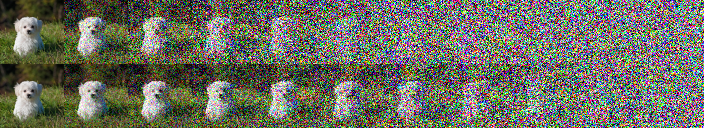
\includegraphics[width=0.8\textwidth]{images/dm/linear_cosine_scheduler}
            $ $\vspace{0.3cm}
            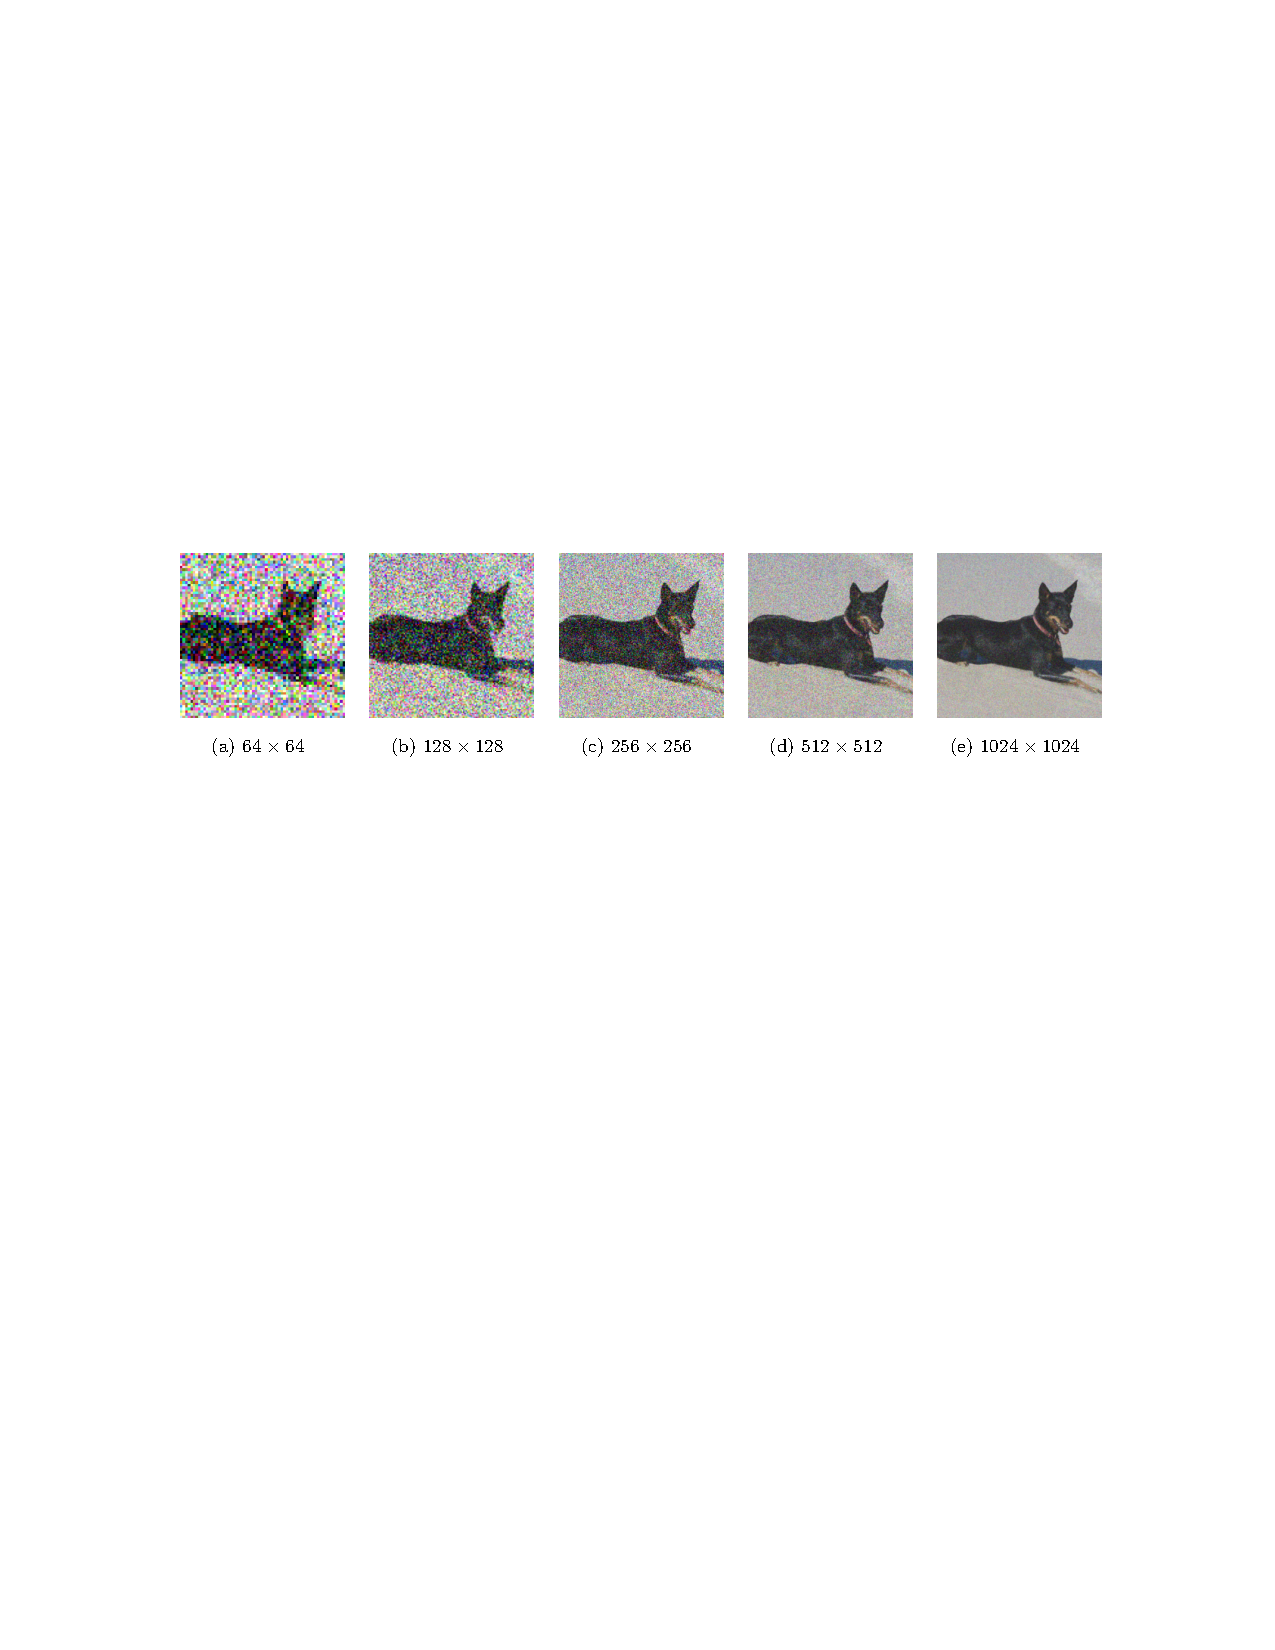
\includegraphics[width=0.8\textwidth]{images/dm/noise_resolution}
            \caption{Imágenes obtenidas desde \cite{nichol2021improved} y \cite{chen2023importancenoiseschedulingdiffusion}.}
        \end{figure}
    }
    \only<2>{
        \insertimage{dm/cyclegan}{1}{Imagen obtenida desde \cite{zhu2020unpairedimagetoimagetranslationusing}.}
    }
    \only<3>{
        \insertimage{dm/short_time}{1}{Imagen obtenida desde \cite{debortoli2023diffusionschrodingerbridgeapplications}.}
    }
\end{frame}

\section{Problema de Schrödinger}

\begin{frame}{Problema de Schrödinger | Notación}

    El problema del puente de Schrödinger ha sido estudiado principalmente desde la matemática, por lo que suele ser formulado, para entregar generalidad, en espacios polacos. Además, hace uso de herramientas de teoría de la medida.

    \begin{itemize}
        \item Por simplicidad, se asumirá que $\xspace=\yspace\subset\R^d$ es compacto.
        \item $\Omega=\mathcal{C}\parent{[0,1],\xspace}$ es el espacio de procesos estocásticos con $t\in[0,1]$.
        \item Si una medida de probabilidad $\mu\in\probmeasure{\xspace}$ tiene función de densidad $p$, entonces $\int_\xspace f(x)\d\mu(x)=\E{x\sim\mu}{f(x)}=\int_\xspace f(x)\,p(x)\d x$.
        \item Si dos medidas de probabilidad $\mu,\nu\in\probmeasure{\xspace}$ tienen función de densidad $p$ y $q$ respectivamente, la derivada de Radon-Nikodym (si es que existe) es $\frac{\d\mu}{\d\nu}(x)=\frac{p(x)}{q(x)}$. En este caso,
        \begin{equation*}
            \KL{\mu}{\nu} = \E{x\sim p(x)}{\log\parent{\frac{p(x)}{q(x)}}} = \int_\xspace \log\parent{\frac{p(x)}{q(x)}} p(x) \d x
        \end{equation*}

    \end{itemize}

\end{frame}

\begin{frame}{Problema de Schrödinger | Formulación dinámica}
    \uncover<1,2>{
        Se puede preferir el problema de buscar un proceso de difusión \textit{natural} que transforme una distribución en otra, en un tiempo finito.
    }
    \uncover<2>{
        \begin{block}{SBP (formulación dinámica)}
            Dadas dos medidas de probabilidad $\mu,\nu\in\probmeasure{\xspace}$ y un proceso estocástico de referencia con ley $R\in\probmeasure{C([0,1],\xspace)}$, el puente de Schrödinger entre $\mu$ y $\nu$ es el (único) proceso estocástico con ley
            \begin{equation*}
                \argmin_{P\in\Gamma(\mu,\nu)} \KL{P}{R} = \E{\omega\sim P}{\log\parent{\frac{\d P}{\d R}(\omega)}},
            \end{equation*}
            donde $\Gamma(\mu,\nu) = \{P\in \probmeasure{C([0,1],\xspace)}: (P_0\sim\mu) \wedge (P_1\sim\nu)\}$ y $\frac{\d P}{\d R}$ es la derivada de Radon-Nikodym (si es que existe).
        \end{block}
    }
\end{frame}

\begin{frame}{Problema de Schrödinger | Formulación dinámica}
    El SBP es similar a los modelos de difusión pero soluciona las limitaciones mencionadas.

    \insertimage{eot_sbp/sbp_solution0.05}{1}{Puente de Schrödinger dinámico entre dos distribuciones discretas. Aquí $R$ es un movimiento browniano.}
\end{frame}

\begin{frame}{Problema de Schrödinger | Formulación dinámica}
    \uncover<1,2>{
    Este problema se puede reformular como un problema de control óptimo:
    \begin{equation*}
        \min_{u\in\mathcal{U}} \E{x}{\int_0^1 \frac{1}{2}\norm{u_t(x)}^2 \d t}
        \quad\text{sujeto a}\quad
        \begin{cases}
            \d x_t = u_t(x) \d t + \d W^\epsilon_t\\
            (x_0\sim\mu) \wedge (x_1\sim\nu),
        \end{cases}
    \end{equation*}
    donde $\mathcal{U}$ es el conjunto de controles admisibles.
    }
\begin{itemize}
    \item<2> Se puede reintrepretar el problema como uno de fluidodinámica cambiando la SDE por su ecuación de Fokker-Planck.
    \item<3> La optimalidad también se puede caracterizar por un sistema acoplado de PDEs. Esto permite entrenar un modelo neuronal para el SBP mediante máxima verosimilitud.
    \item<4> En este caso, la función objetivo generaliza a la de los modelos de difusión a tiempo continuo.
\end{itemize}

\end{frame}

\begin{frame}{Problema de Schrödinger | Formulación estática}
    \uncover<1>{
        Se puede demostrar la siguiente descomposición:
        \begin{equation*}
            \KL{P}{R} = \KL{P_{01}}{R_{01}} + \E{(x,y)\sim P_{01}}{\KL{P_{|xy}}{R_{|xy}}}.
        \end{equation*}
    }
    \uncover<2>{
        Luego, el SBP dinámico se puede reducir a un problema estático enfocado únicamente en los extremos del proceso:
        \begin{equation*}
            \underbrace{\min_{P\in\Gamma(\mu,\nu)} \KL{P}{R}}_{\text{problema dinámico}} = \underbrace{\min_{P_{01}\in\Pi(\mu,\nu)} \KL{P_{01}}{R_{01}}}_{\text{problema estático}},
        \end{equation*}
        donde $\Pi(\mu,\nu) = \{\pi\in\probmeasure{\R^d\times\R^d}\,: (\pi_0\sim\mu) \wedge (\pi_1\sim\nu)\}$.
    }

    \uncover<3>{
        Por lo tanto, si $P_{01}^*$ es la (única) solución del SBP estático, la (única) solución del SBP dinámico es
        \begin{equation*}
            P^*(\cdot) = \int_{\xspace\times\xspace} R_{|xy}(\cdot) \d P_{01}^*(x,y).
        \end{equation*}
    }
\end{frame}


\begin{frame}{Problema de Schrödinger | Formulación estática}
    \uncover<1,2>{
        En particular, si $R$ es el movimiento browiano con difusividad $\epsilon$, el problema estático se reduce al problema de EOT estándar.
    }
    \uncover<2>{
        \begin{align*}
             & \KL{P_{01}}{W_{01}^\epsilon}\\
             & \quad = \frac{1}{\epsilon}\rparent{\underbrace{\int_{\xspace\times\xspace} \frac{1}{2} \norm{x-y}^2 \d P_{01}(x,y)}_{\text{costo de transporte}} + \underbrace{- \epsilon\cdot\entropy{P_{01}}}_{\text{regularizador}}} + \cte,
        \end{align*}

        donde $\entropy{P_{01}}$ es la entropía (diferencial) de $P_{01}$.
    }

    \uncover<3>{
        Más aún, todo SBP (con una cierta medida de referencia) puede ser transformado a un problema de EOT (con una cierta función de costo), y viceversa.
    }

\end{frame}

\begin{frame}{Problema de Schrödinger | Formulación dinámica}
    \insertimage{eot_sbp/discrete_sinkhorn_graph0.1}{1}{Puente de Schrödinger estático entre dos distribuciones discretas.}
\end{frame}

\section{Transporte óptimo}

\begin{frame}{Transporte óptimo | Problema de Monge}
    \uncover<1,2>{
        El problema de transformar una distribución en otra puede modelarse como un problema de transporte óptimo:
        \begin{center}
            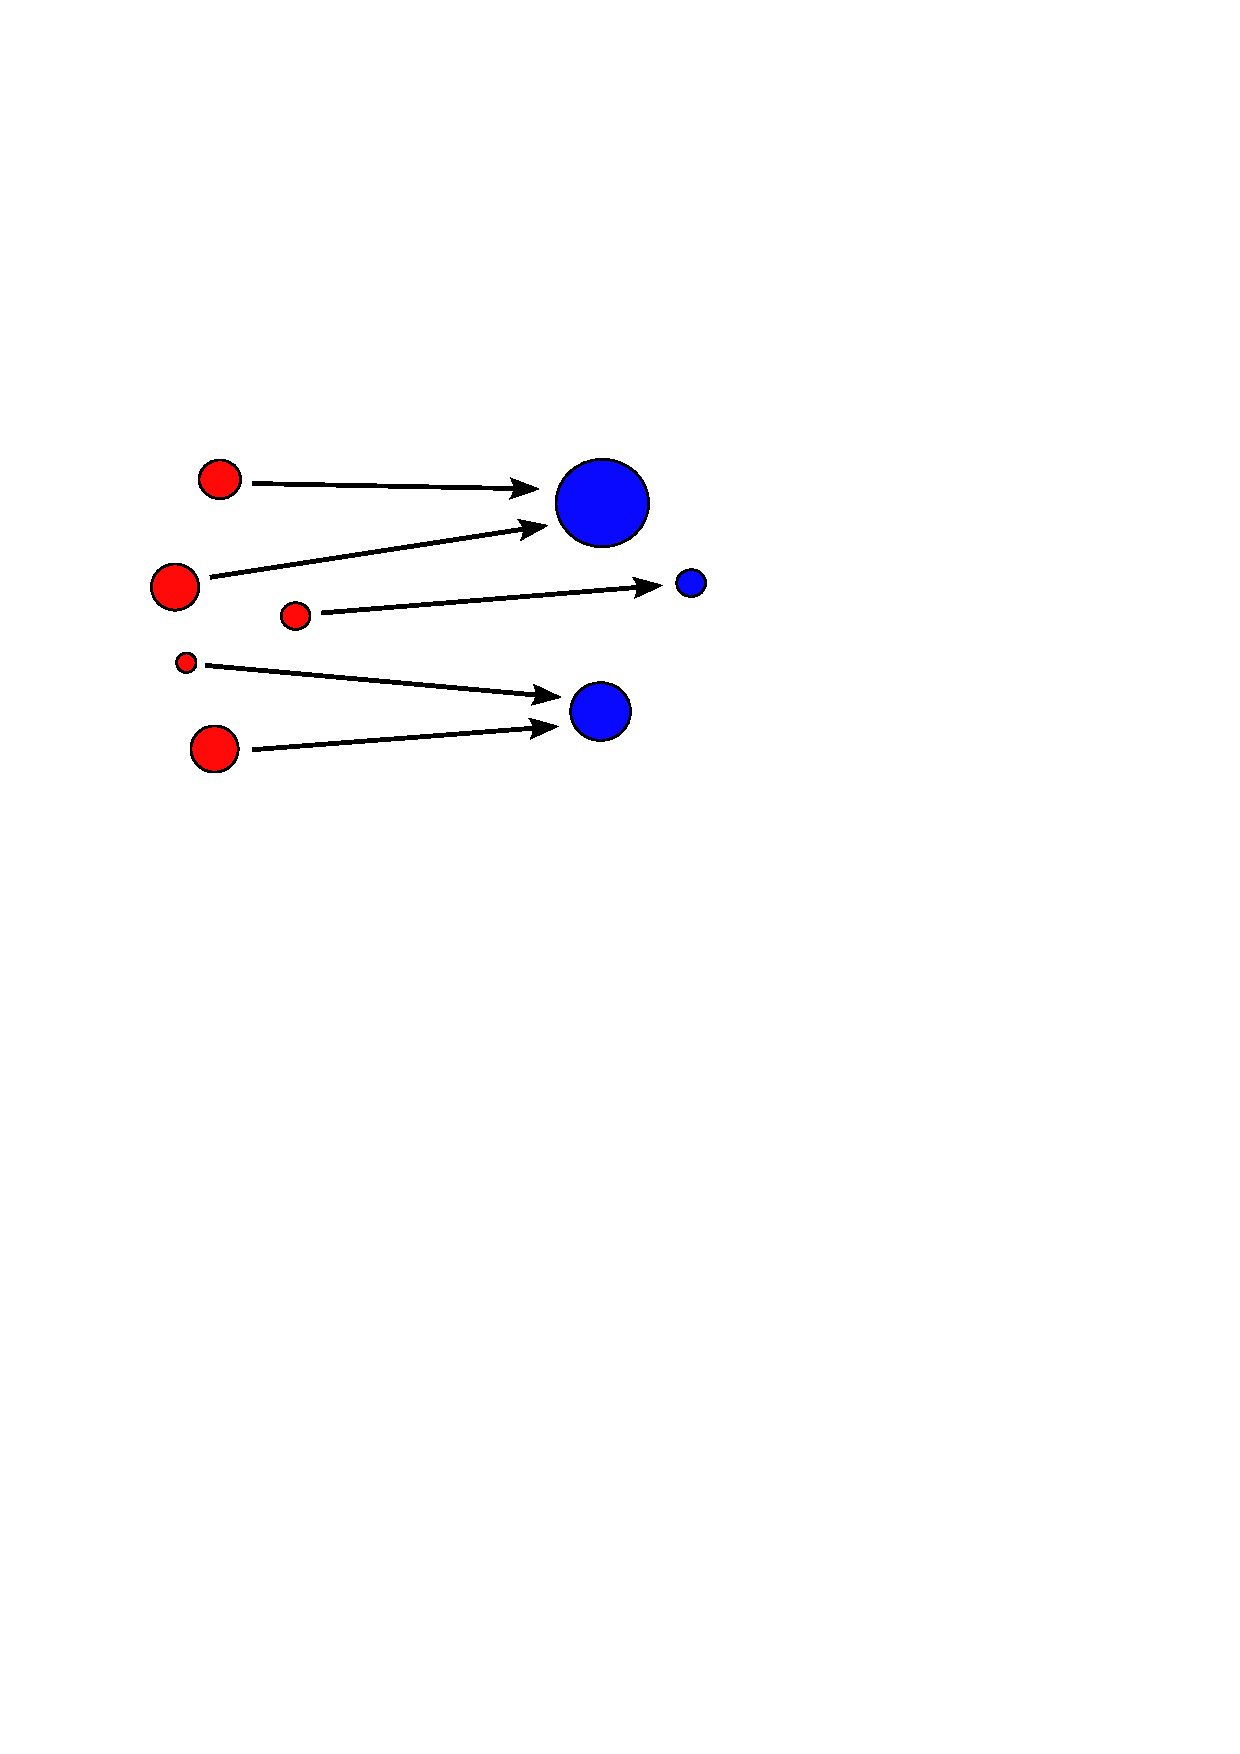
\includegraphics[width=0.3\textwidth]{images/ot/monge_discrete}
            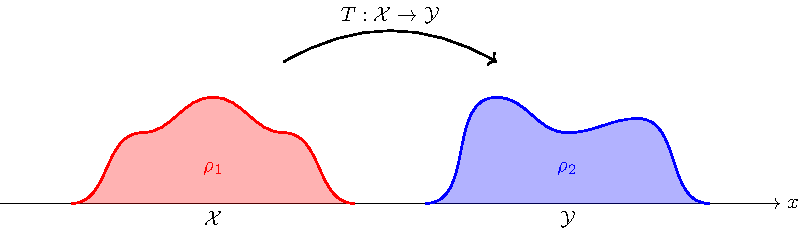
\includegraphics[width=0.69\textwidth]{images/ot/earth_mover}
        \end{center}
    }
    \uncover<2>{
        \begin{block}{Problema de Monge}
            Si $c:\xspace\times\yspace\to\R_+$ es una función continua que mide la \textit{discrepancia} entre dos puntos, el problema de Monge entre $\mu\in\probmeasure{\xspace}$ y $\nu\in\probmeasure{\yspace}$ es:
            \begin{equation*}
                \inf_{\feasible{T:\xspace\to\yspace}{T_\#\mu=\nu}}
                \int_{\xspace} c(x, T(x)) \d\mu(x),
            \end{equation*}
            donde la igualdad $T_\#\mu=\nu$ indica que $T(x)\sim\nu$ cuando $x\sim\mu$.
        \end{block}
    }
\end{frame}

\begin{frame}{Transporte óptimo | Relajación de Kantorovich}
    \uncover<1,2>{
        El problema de Monge es altamente no lineal, no es convexo ni posee necesariamente solución.
    }

    \visible<2>{
        Estas limitaciones se pueden suprimir si se permite división de masa.

        \begin{columns}
            \begin{column}{0.49\textwidth}
                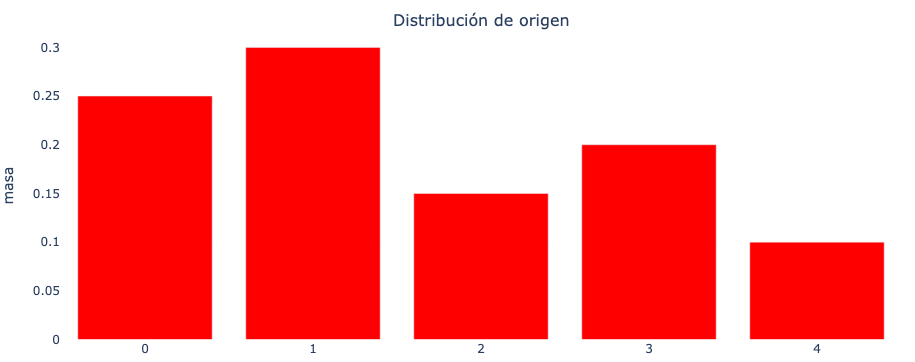
\includegraphics[width=\textwidth]{images/ot/kantorovich_discrete_histogram1}
                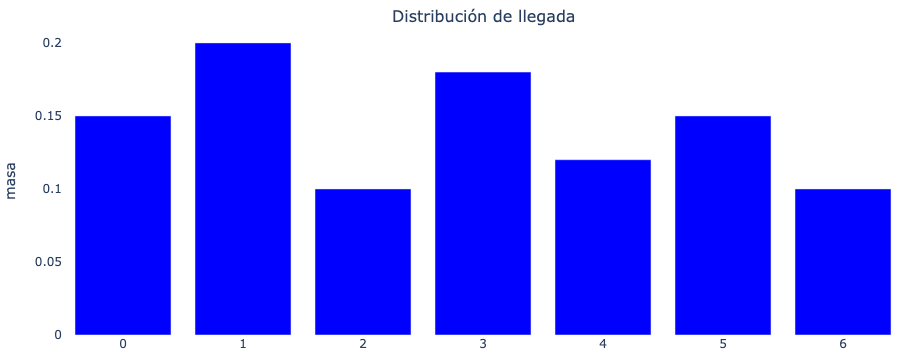
\includegraphics[width=\textwidth]{images/ot/kantorovich_discrete_histogram2}
            \end{column}
            \begin{column}{0.5\textwidth}
                % Resuelto usando SciPy.
                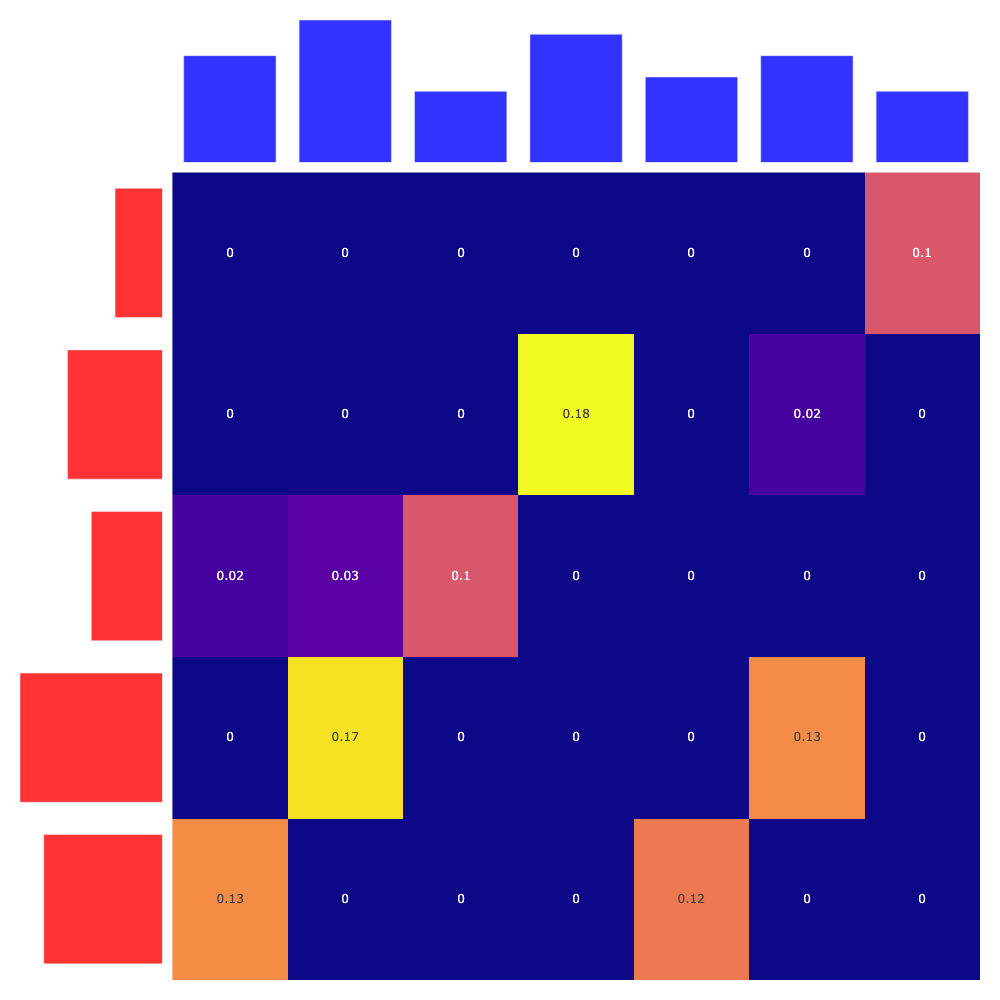
\includegraphics[width=\textwidth]{images/ot/kantorovich_discrete_solution}
            \end{column}
        \end{columns}
    }

\end{frame}

\begin{frame}{Transporte óptimo | Relajación de Kantorovich}
    \uncover<1->{
        \begin{block}{Relajación de Kantorovich}  % c convexa?
            Si $c:\xspace\times\yspace\to\R_+$ es una función continua que mide la \textit{discrepancia} entre dos puntos, el problema de Kantorovich entre $\mu\in\probmeasure{\xspace}$ y $\nu\in\probmeasure{\yspace}$ es:
            \begin{equation*}
                \inf_{\pi \in \Pi(\mu,\nu)} \int_{\xspace\times\yspace} c(x, y) \d\pi(x, y),
            \end{equation*}
            donde $\Pi(\mu,\nu) = \{\pi\in\probmeasure{\xspace\times\yspace}\,: \pi_0=\mu, \pi_1=\nu\}$.
        \end{block}
    }
    \begin{itemize}
        \item<2> Es un problema convexo y cumple dualidad fuerte.
        \item<3> Este problema, más un término regularizador, equivale al SBP estático.
    \end{itemize}

\end{frame}

\begin{frame}{Transporte óptimo | Relajación de Kantorovich}
    \begin{columns}
        \begin{column}{0.44\textwidth}
            Bajo hipótesis razonables, ambos problemas son equivalentes en el caso continuo: si $\pi^*\in\probmeasure{\xspace\times\yspace}$ es la solución del problema de Kantorovich, toda su masa está concentrada en una curva, que resulta ser el grafo de la solución $T^*:\xspace\to\yspace$ del problema de Monge.
        \end{column}
        \begin{column}{0.55\textwidth}
            % Usando POT.
            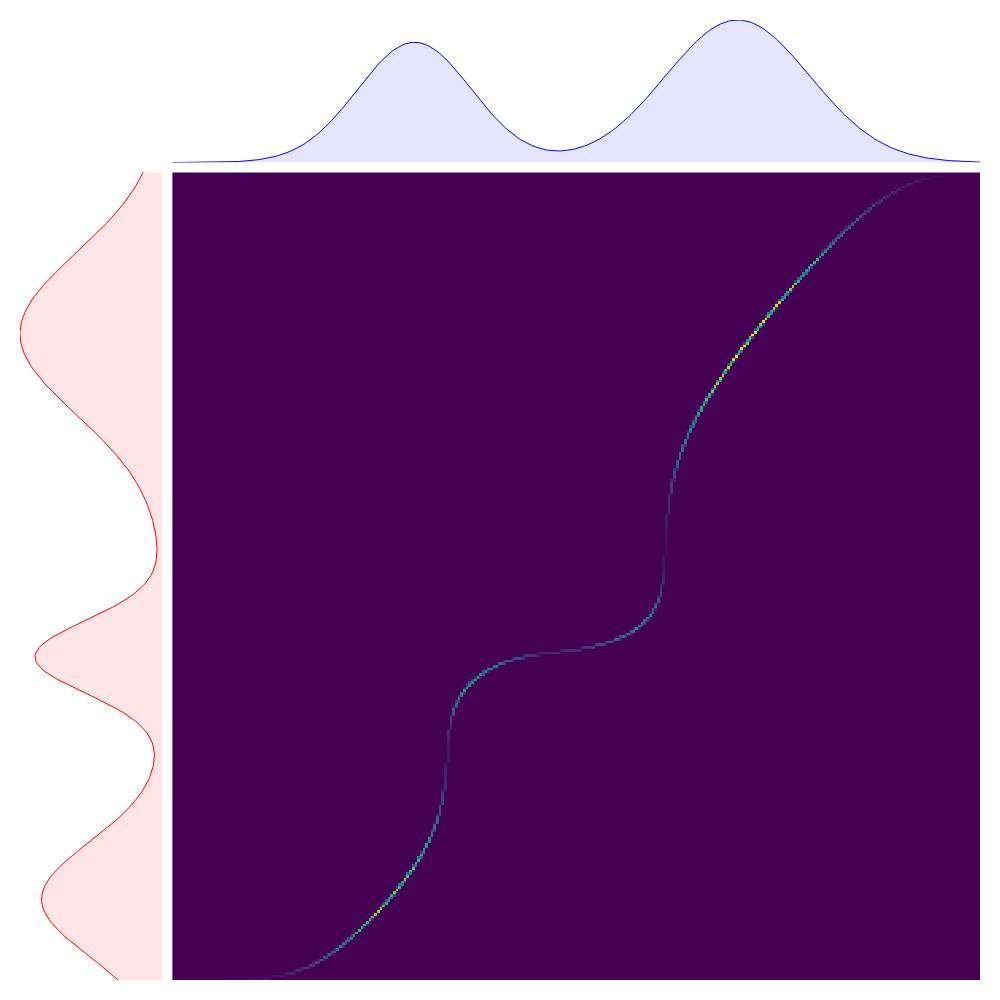
\includegraphics[width=\textwidth]{images/ot/kantorovich_continuous_solution}
        \end{column}
    \end{columns}
\end{frame}

\begin{frame}{Transporte óptimo | Distancia de Wasserstein}
    \uncover<1>{
    Si $d:\xspace\times\xspace\to\R_+$ es una distancia en $\xspace$, entonces
    \begin{equation*}
        \wasserstein{p}{\mu,\nu} = \parent{\inf_{\pi\in\Pi(\mu,\nu)}\int_{\xspace\times\xspace} d(x,y)^p\d\pi}^{\frac{1}{p}}
    \end{equation*}
    es una distancia en $\probmeasure{\xspace}$, llamada \textit{distancia de Wasserstein}.
    }

    \only<2>{
        El espacio métrico $\parent{\probmeasure{\xspace},\mathcal{W}_p}$ es geodésico. Esto permite obtener una formulación dinámica del transporte óptimo. %, obteniendo una dualidad estático-dinámica similar al SBP.

    \insertimage{ot/distr_transform}{1}{Imagen obtenida desde...}
    }
\end{frame}

\begin{frame}{Transporte óptimo | Distancia de Wasserstein}
    \only<1>{
    Esta distancia permite interpolar entre distribuciones de probabilidad a través de geodésicas en $\probmeasure{\xspace}$, generando interpolaciones más realistas que la interpolación euclidiana.
    \begin{center}
        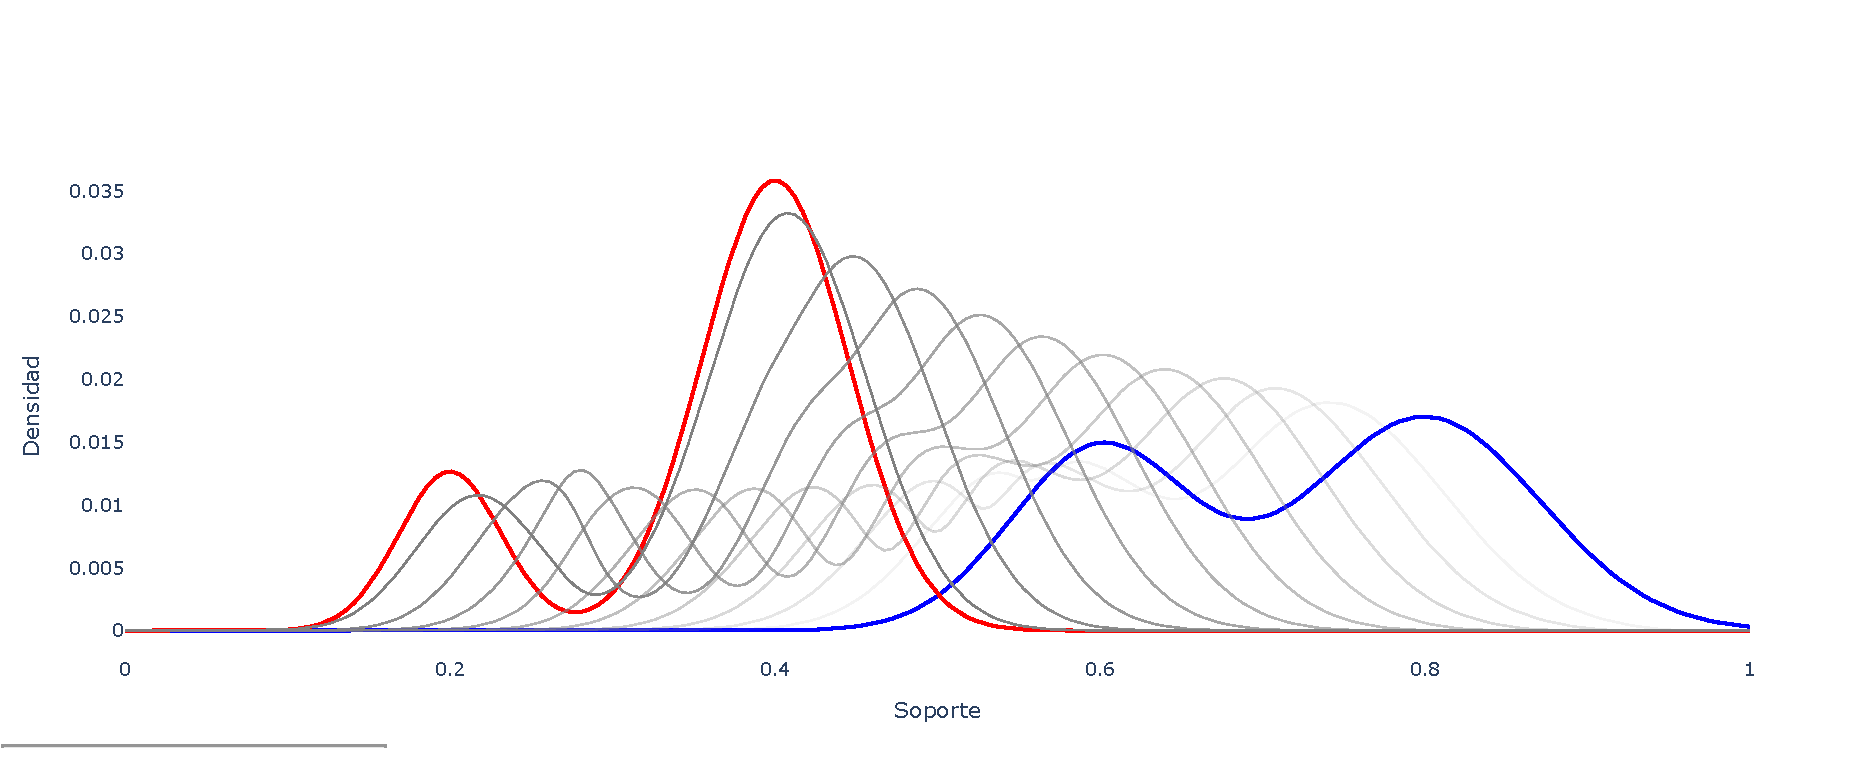
\includegraphics[width=0.8\textwidth]{images/ot/gmm_interpolation}
        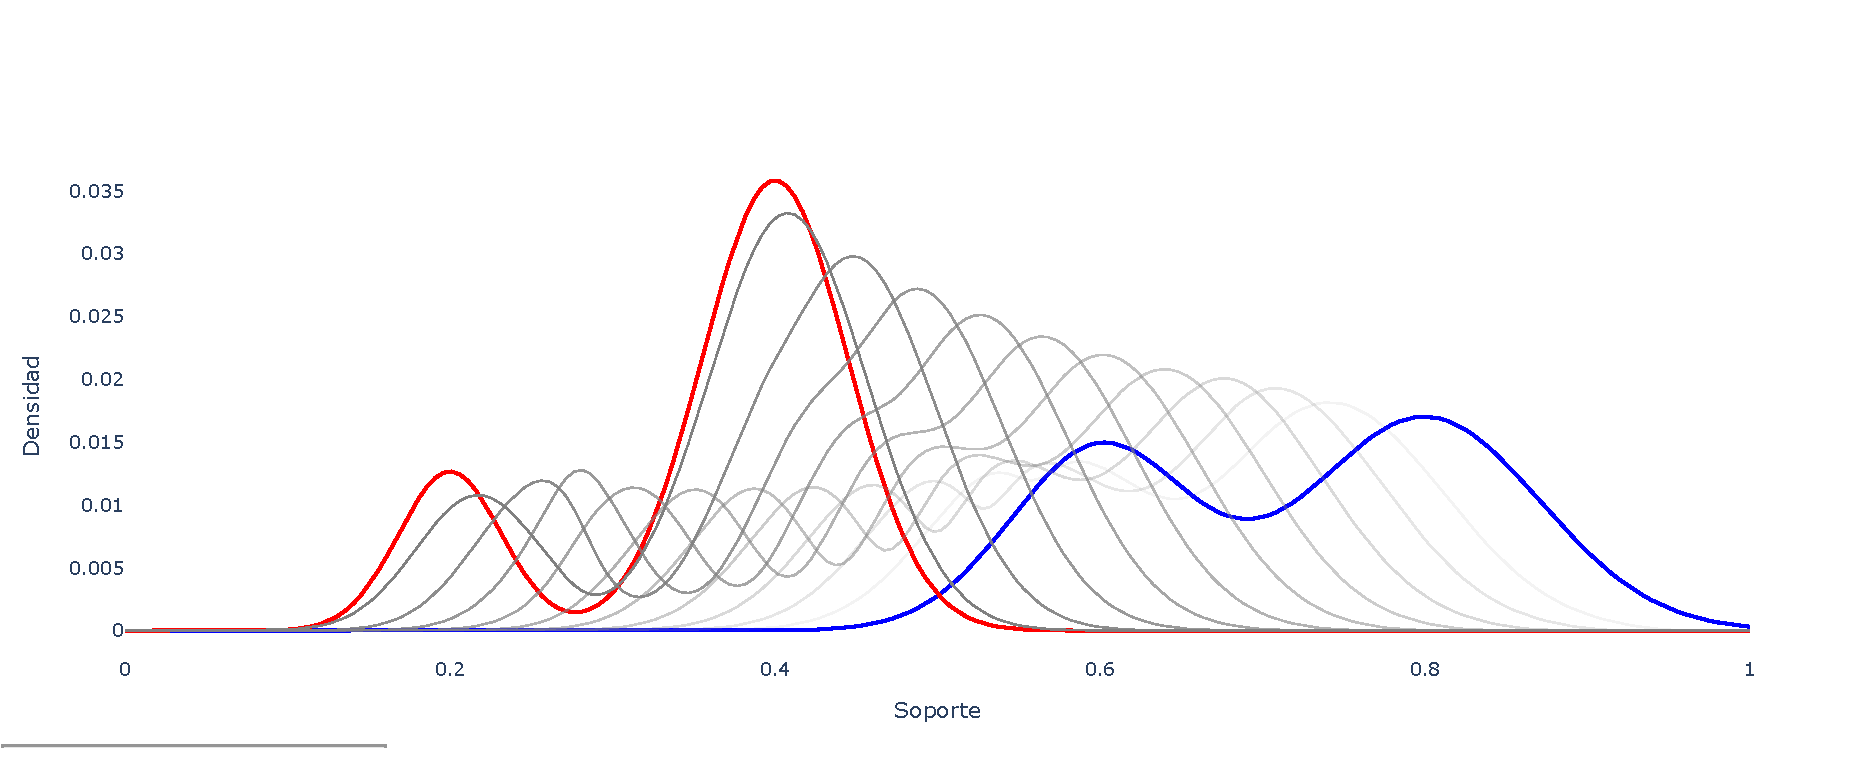
\includegraphics[width=0.8\textwidth]{images/ot/gmm_interpolation}
    \end{center}
    }
\end{frame}

\begin{frame}{Transporte óptimo | Distancia de Wasserstein}
    Más aún, se puede realizar interpolación baricéntrica de forma eficiente:
    \begin{center}
        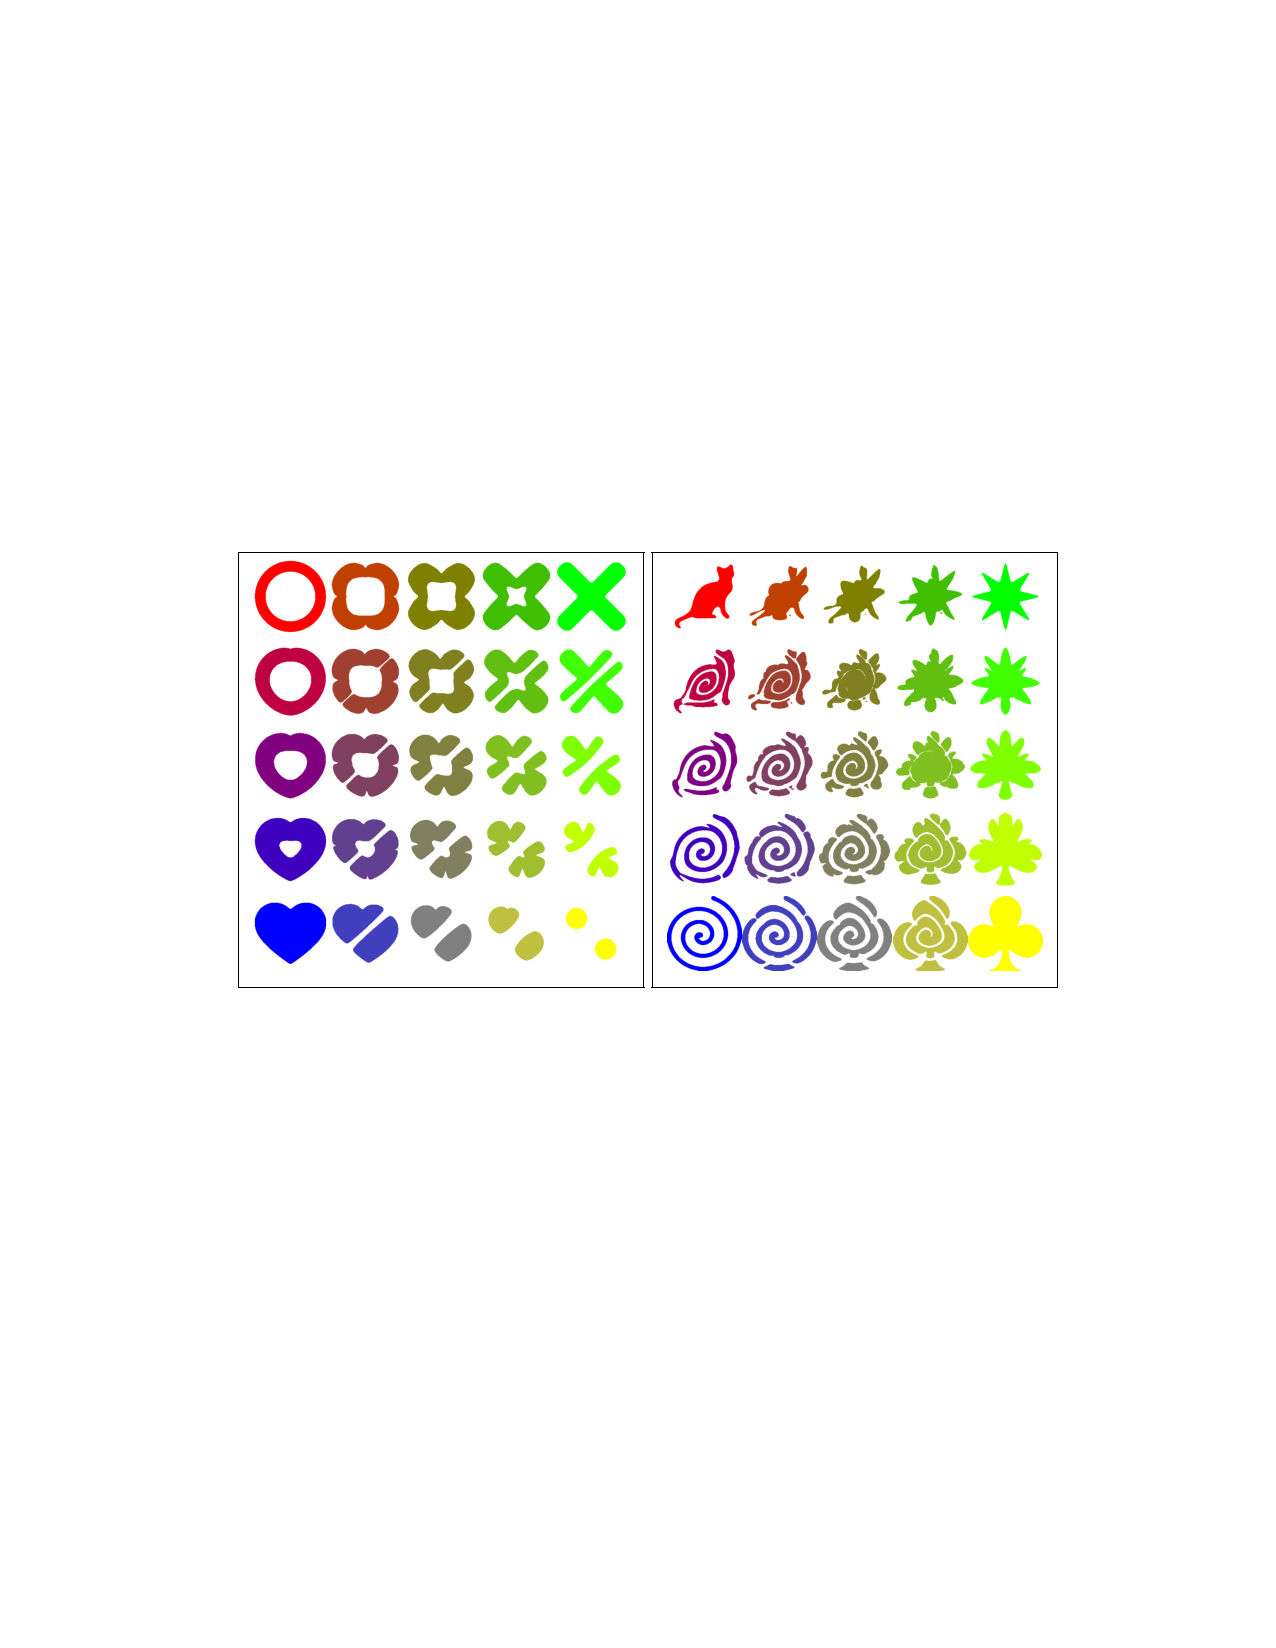
\includegraphics[width=0.9\textwidth]{images/ot/barycenter}
    \end{center}
\end{frame}
    
\begin{frame}{Transporte óptimo | Distancia de Wasserstein}
    La distancia de Wasserstein tiene buenas propiedades matemáticas:
    \begin{itemize}
        \item<1> Es más débil que la distancia en variación total. Más aún, metriza la convergencia débil de medidas.
        \item<2> Puede ser optimizada por redes neuronales: si $g_\theta(z)\sim\mu_\theta$ es un modelo generativo neuronal de variable latente $z\sim\gaussian{0}{\identity{l}}$,  entonces $\theta\mapsto\wasserstein{1}{\mu_\theta,\mu_{\text{true}}}$ es diferenciable (c.t.p.).
        \item<4,5> El problema se puede reformular como uno de control óptimo:
        \begin{equation*}
        \min_{u\in\mathcal{U}} \E{x}{\int_0^1 \frac{1}{2}\norm{u_t(x)}^2 \d t}
        \quad\text{sujeto a}\quad
        \begin{cases}
            \d x_t = u_t(x) \d t\\
            (x_0\sim\mu) \wedge (x_1\sim\nu),
        \end{cases}
    \end{equation*}
    donde $\mathcal{U}$ es el conjunto de controles admisibles.
        \item<5> Formulación de Benamou-Brenier: se puede sustituir la dinámica de $x$ por la ecuación de continuidad, transformando el problema en uno de fluidodinámica.
    \end{itemize}
\end{frame}

\begin{frame}{Transporte óptimo | Modelos de difusión como OT}

    \begin{columns}
        \begin{column}{0.39\textwidth}
            \insertimage{ot/dm_ot}{1}{Imagen obtenida desde }
        \end{column}
        \begin{column}{0.6\textwidth}
            \begin{itemize}
                \item<1> Para un modelo de difusión hasta tiempo $T>0$, se denotará por $E_{T}(x)\in\yspace$ el lugar al que llega un punto $x\sim\ptrue(x)$ que fluye a través de la \textit{probability flow ODE}.
                \item<2> Se ha probado empíricamente que $E_T$ también converge al mapa de Monge entre $\ptrue$ y $\pprior$.
                \item<3> Se han dado contraejemplos teóricos donde esto no ocurre.
            \end{itemize}
        \end{column}
    \end{columns}

\end{frame}

\end{document}